\documentclass[../Main.tex]{subfiles}

\begin{document}

\begin{tcolorbox}[colback=light-orange, boxrule=0pt]
  \begin{multicols}{3}
%\begin{minipage}[t]{0.65\textwidth}\vspace{0pt}
   \textcolor{blue}{\textbf{ABSTRACT:}} Pythoplankton blooms in Baltic are annual event in the Batlic. They mostly occure in spring and fall during the year.[BASIC INTRODUCTION]
   To understand the dynamics of pythoplankton blooms, many factors from light to temperature were investigated before. Mostly 
 The factors that potentially drive pythoplankton blooms were investigated from many points of view [MORE DETAILED BACKGROUND]
Mostly the data for getting the assumptions about the pythoplankton bloom are lacking on accuary and continuaty [GENERAL PROBLEM]
Here we show an overview about a new high resolution dataset recorded by a glider in the Baltic from March to Octorber in 2021.[HERE WE SHOW...]
[MAIN RESULT]
[GENERAL CONTEXT]
%\end{minipage}
%\begin{minipage}[t]{0.3\textwidth}\vspace{0pt}
  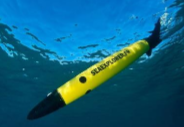
\includegraphics[width=0.3\textwidth, center]{Glider.png}
  %\end{minipage}
  \end{multicols}
\end{tcolorbox}
\end{document}
